\chapter{Memory organization}

Larger memories are slower than smaller memories.
Fast memories are much more expensive than slow memories.

So instead of using a single large memory, modern systems use a hierarchy. 
Characterized by different technology, cost, dimensions and access mechanisms. The programmer sees an unique large memory space. The CPU sees a fast memory at acceptable cost.

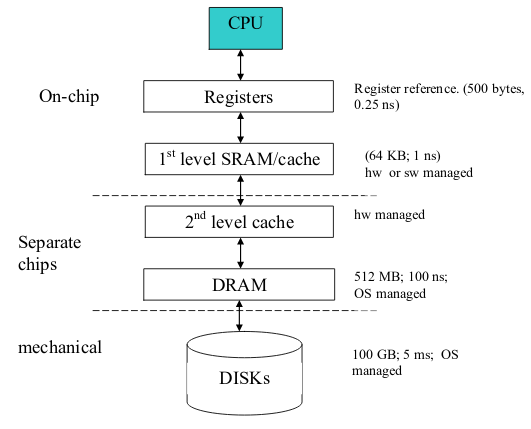
\includegraphics[width=.7\textwidth]{images/memory_hierarchy.png}
Hierarchies work well because memory access follows the principle of locality.

\paragraph{Locality}
\begin{itemize}
    \item \textbf{Temporal locality}:\\
    when a memory entry is referenced, with high probability it will be referenced again within a short time.
    
    \item \textbf{Spatial locality}:\\
    whenever a memory entry is referenced, with high probability reference will be made shortly to neighboring items.
\end{itemize}

\paragraph{Registers}
Registers are usually “exposed” to the programmer. Alternatively, the compiler allocates variables to registers.
Registers are usually placed into a regular register file. A register file consists of multiple read/write ports to allow parallel, simultaneous data accesses.
Typically, at least 2 read and 1 write ports are required to access operands of a single instruction.

Unfortunately, the size of the register file grows with the square of the number of ports so an excessive number of ports slows down the processors.

This quadratic increase in chip area is mostly due to the new additional input and output lines:\\
• Routing problems\\
• Internal bit cell loading increases -> larger power consumption\\
• Linear increment in delay with the number of ports

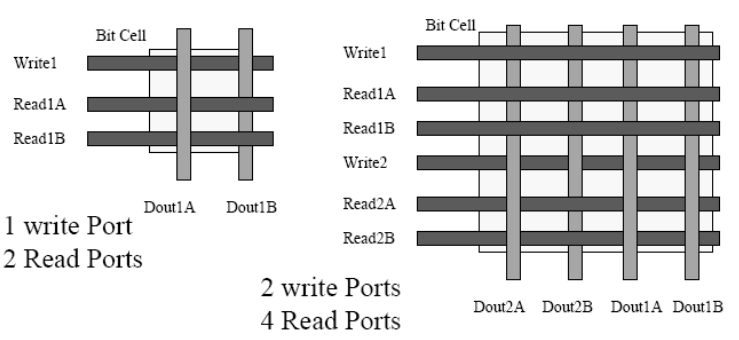
\includegraphics[width=.7\textwidth]{images/memory_bit_cells.png}

It is not profitable to have a register file with more than 15-20 ports: 12 is actually the best tradeoff when number of FU is larger than 4

\paragraph{The usual SRAM}
\begin{itemize}
    \item It is “exposed” to programmer and compiler
    \item Data transfers from/to memory are performed by \textbf{software}
    \item It is mostly used in low-end or specialized embedded processors where worst-case latency to recover data and power are the main issues
\end{itemize}

\paragraph{Cache}
\begin{itemize}
    \item Usually it is “transparent” to programmer and compiler
    \item Transfers from/to lower-level memories are performed by \textbf{hardware}
    \item It is mostly used in high-end processors where the power is less critical and average performance should be maximized
\end{itemize}

\paragraph{Scratch Pad}
It's a low power consumption solution.
The scratch pad is a buffer of memory (no cache) where most frequently used program functions instructions and data are allocated.
This approach requires a preliminary “profiling”to decide what instructions have to be placed into the scratch pad.
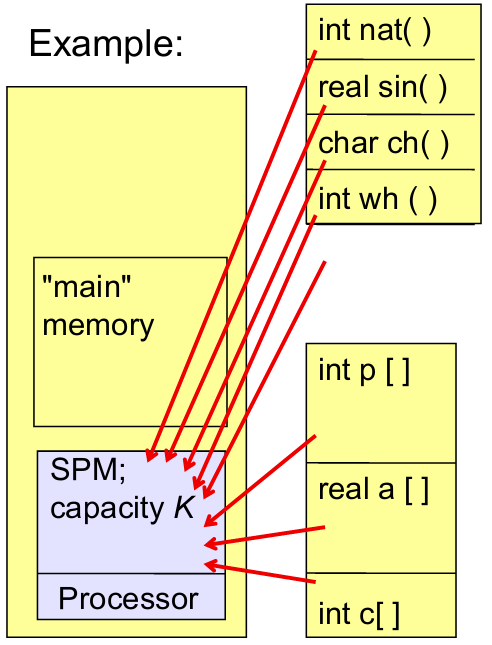
\includegraphics[width=.5\textwidth]{images/memory_scratch_pad.png}
Allocation usually performed statically at compile time (no HW support).
This kind of solution is very used in embedded systems because the program is usually fixed and it is a reasonable tradeoff between performance and power consumption.

\paragraph{Cache}
A cache is a special kind of memory based on SRAM cells which is used to store the data having the maximum probability to be used.
Cache can be either unified (i.e., simultaneously instruction-and data-cache) or split into I-cache and D-cache.

Definitions:
\begin{itemize}
    \item \textbf{Hit}: the item requested by the CPU is present in cache
    \item \textbf{Miss}: the item requested by the CPU is not present in cache
    \item \textbf{Hit rate}: fraction of memory accesses rewarded by hit
    \item \textbf{Miss rate}: fraction of memory accesses resulting in a miss (miss rate = 1 -hit rate)
    \item \textbf{Hit time}: access time (or clock cycles) to cache in the case of success (includes time to determine whether access is met by hit or miss)
    \item \textbf{Miss penalty}: time (or clock cycles) required to substitute a block of data in cache with another block from the lower-level storage
    \item \textbf{Miss time}: miss penalty + hit time, time required to obtain requested data in the case of miss
\end{itemize}

Cache performance is given in terms of average memory access time (AMAT)

$AMAT = hit-time + miss-rate * miss-penalty$\\

Cache performance affects CPU time

$CPU_{time} = IC * (CPI_{execution} + \frac{MEM_{accesses}}{IC} * miss-rate * miss-penalty) * T_{CLK}$

\paragraph{How cache works}
A cache is made of a number of \textbf{blocks} that contain \textbf{words} from memory.
The size of a block is a power of 2, to simplify addressing (e.g., a block is made of 32 words).
When a word is needed, its entire block is loaded from memory and placed somewhere in the cache.
Blocks that are next to each other in memory are not necessarily stored next to each other in the cache, and vice-versa.

The cache needs to store a block along with its actual address in memory.
The required address is compared to the address of all the blocks in the cache to find a match.
If found, it is a hit, otherwise it is a miss.

\paragraph{Problems in cache design}
\begin{itemize}
    \item \textbf{Placement problem}:\\
    Where to place a block transferred from lower to higher level
    \item \textbf{Search (or identification) problem}:\\
    how to determine whether the requested item is present or not
    \item \textbf{Substitution (or replacement) problem}:\\
    Which block present in the cache must be replaced by one in lower-level storage, in the case of a miss
    \item \textbf{Write strategy}:\\
    what happens when a write-to-memory instructions is executed?
\end{itemize}

\section{Direct-mapped cache}
Assume the cache is made of an array of $N_B$ blocks.
Let $B_{AR}$ be the address of the required block in RAM.

In a direct-mapped cache, the block can only be placed in the cache block at address $B_{AC}$:

$B_{AC} = B_{AR} mod N_B$

$B_{AC}$ is also called the index of the cache block.
If $N_B$ is a power of 2, then the index is equal to the $N_{AC} = log2(N_{B}$ least significant bits of $B_{AR}$.

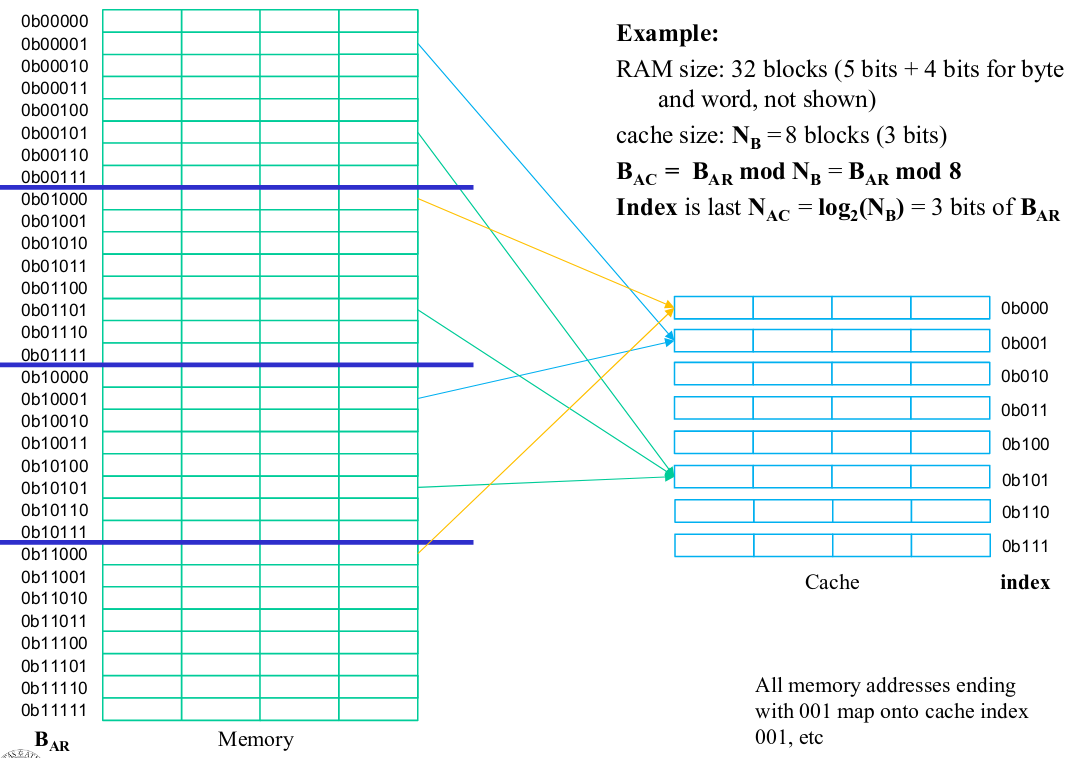
\includegraphics[width=\textwidth]{images/direct_mapped_cache.png}

\paragraph{Problems}
\begin{itemize}
    \item \textbf{Placement problem}:\\
    Trivial – the block from RAM can be mapped onto one cache block only
    \item \textbf{Search problem}:\\
    different memory blocks can be placed in the same cache block. How do we decide which location is mapped in the cache?\\
    \textbf{Solution}: each cache line must be provided with:
    \begin{itemize}
        \item A \textbf{tag field} containing the $N_{AR} - N_{AC}$ most significant bits of $B_{AR}$
        \item A \textbf{validity bit} - denotes whether block contains meaningful (valid) data.
    \end{itemize}
    \item \textbf{Replacement problem}:\\
    Trivial – the new block from RAM can be mapped onto one cache block only. Does not account for temporal locality! Block substituted may have been very recently used.
\end{itemize}

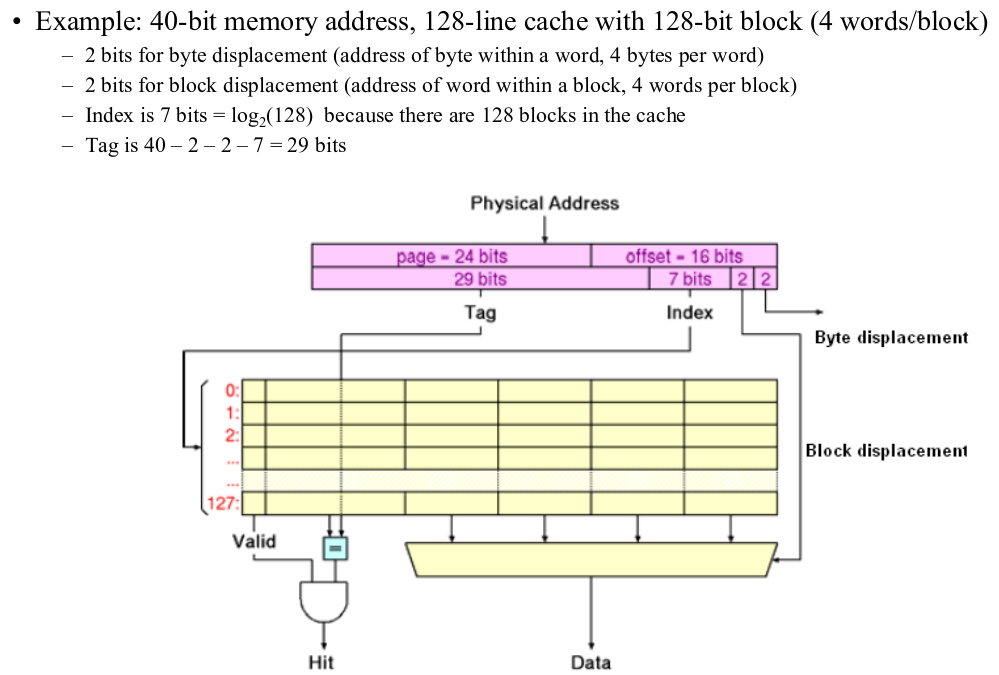
\includegraphics[width=\textwidth]{images/direct_mapped_cache_example.png}

\section{Fully associative cache}
In fully-associative cache every block of RAM can be mapped onto any block of cache (there is no constraint on Placement).
The search problem is tackled by running a parallel comparison of  the wanted address with all tags. So a large number of comparators is done and so it's very expensive in terms of area and power consumption.

The index is 0 bits and the tag is the complete address of the word minus the bits for block and byte displacements. 

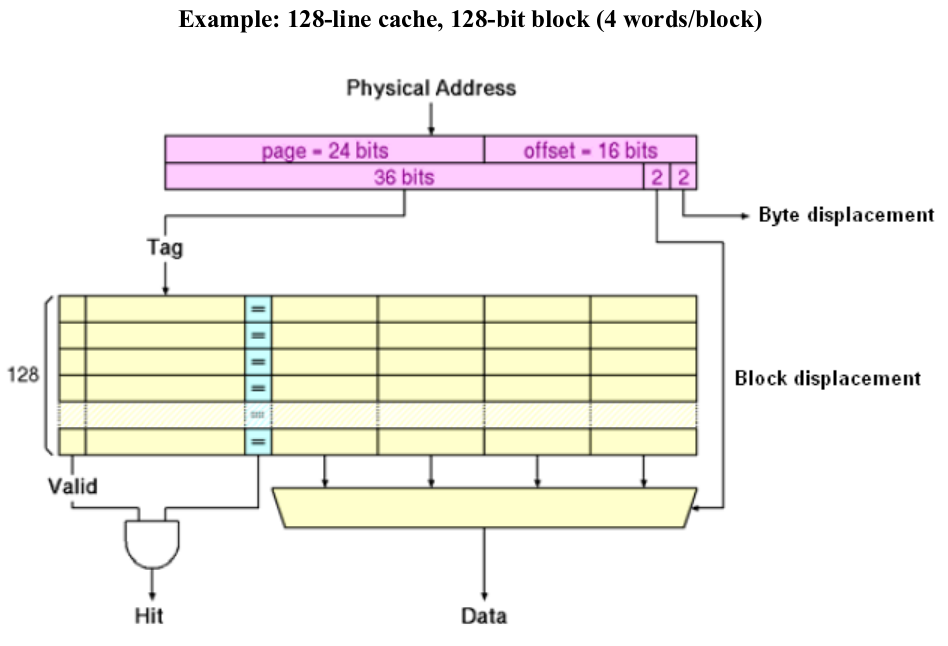
\includegraphics[width=\textwidth]{images/fully_associative_cache.png}

\paragraph{Replacement strategies}
\begin{itemize}
    \item \textbf{Random}:\\
    the block to be substituted is chosen randomly.
    \begin{itemize}
        \item \textit{pro}: It is simple. Minimum HW support (pseudo-random number generator)
        \item \textit{cons}: Efficiency in terms of miss rate is comparable to DM cache. In fact, temporal locality not taken into account.
    \end{itemize}
    \item \textbf{Least Recently Used (LRU)}:\\
    substitute the block left unused for the longest time.
    \begin{itemize}
        \item \textit{pro}: It fully exploits temporal locality. Maximum efficiency
        \item \textit{cons}: It requires HW support. The cost of this solution increases largely with the number of blocks. A counter per each block.
    \end{itemize}
    \item \textbf{First In First Out (FIFO)} (also called Round Robin) of length N:\\
    substitute the block used N accesses before the present one. Whether it was used during the last N-1accesses or not.
    \begin{itemize}
        \item \textit{pro}: This is the best tradeoff between performance and complexity. It is adopted in several recent systems.
        \item \textit{cons}: It just approximates the locality principle
    \end{itemize}
\end{itemize}

\section{N-way set-associative cache}
N-way set-associative cache is a tradeoff between DM and fully associative solutions.
Cache is arranged in $N_{set}$ sets ($N_{set}$ being a power of 2), each set including N blocks. Notice:  $N_{set} = N_B/ N$   where $N_B$ is the total number of blocks.

The index $I_{set}$ of the Set in cache corresponding to a given memory block address $B_{AR}$ is given by:\\
$I_{set} = B_{AR} mod N_{set}$

Each block within the set at index  $I_{set}$ can map onto any of the N cache blocks in the set, using fully associative technique.

The set in cache corresponding to block in RAM is identified as in DM cache (Index identifies Set). Within the set, block is identified with associative mechanisms (multiple tag comparisons in parallel).

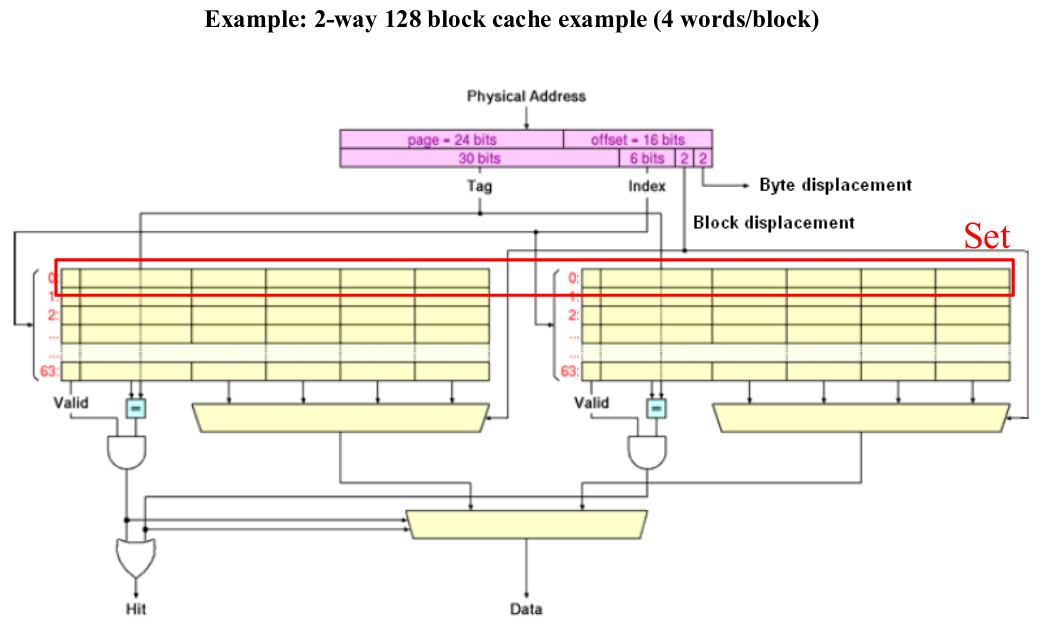
\includegraphics[width=\textwidth]{images/n-way_set_associative.png}

The direct mapped cache is a 1-way set associative cache (set = 1 block).
The fully associative cache has only one big set, the size of the whole cache.

\textbf{Advantages compared to fully associative cache}: comparators are fewer and smaller so cheaper and faster solutions.

\textbf{Advantages compared to direct-mapped cache}: better exploitation of temporal locality at a reasonable cost

The replacement of a block is performed by one of the techniques seen for associative cache (random, LRU or round-robin).

\section{Causes of cache miss}
\begin{itemize}
    \item \textbf{Compulsory misses}:\\
    at the time of the first access, a block is never present in cache. Not dependent on cache size and architecture (dependent on block size, though)
    \item \textbf{Capacity misses}:\\
    if the cache cannot contain all the blocks needed during execution of a program, capacity misses will occur due to blocks being discarded and later retrieved. This kind of misses decreases with cache size
    \item \textbf{Conflict misses}:\\
    in direct-mapped or set-associative caches, blocks that are replaced may have to be reloaded later in the same set – leading to collision (“conflict”) misses
\end{itemize}

\subsection{The write problem}
Write in caches are less frequent than reads.
Instruction fetch only requires memory reads.
“Load” instructions more frequent than “store”.

In Write to memory operations we ask:
\textbf{Speed}: implies writing to cache;
\textbf{Consistency}: information in lower-layer memories must always be consistent with information in cache.

\subsubsection{Write strategies:}
\paragraph{Write-through}
information is written \textbf{simultaneously} in cache block and in the main memory block. Consistency always respected, access time for writes is that of the lower level of memory, so lower performance.

\paragraph{Write-back}
when a write instruction is executed, data are written \textbf{only in a cache} block. Lower-level memory block is modified instead \textbf{only when a substitution occurs}.

It's added a "dirty bit" to specify if the cache block is dirty or clean, so if the data is useful.

Generally, write-back is preferred to write-through because locality principle leads to high probabilities of writing again in a block recently accessed for a write. So there is a good probability of multiple writes before a substitution occurs.

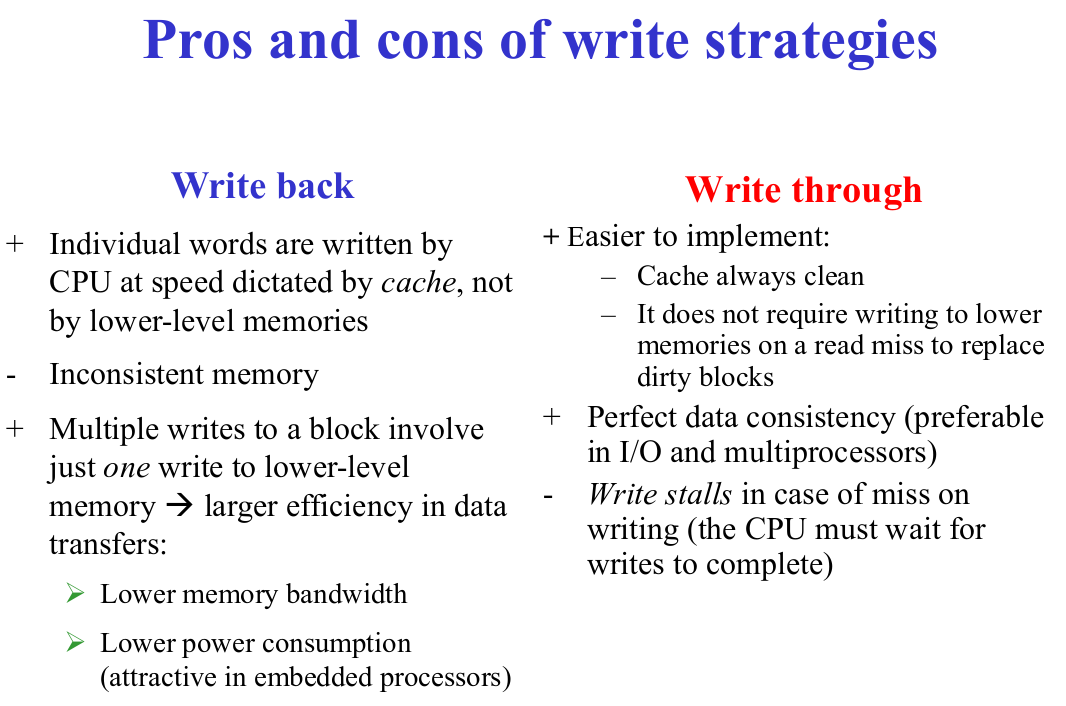
\includegraphics[width=\textwidth]{images/write_strategies.png}

\paragraph{Improving the efficiency of write through}
In order to reduce the latency due to write stalls, a write buffer between cache and lower-layer memory is inserted. CPU writes to cache and write buffer. The write buffer is a simple FIFO.
Data are transferred from CPU to buffer at cache speed, and from buffer to memory at memory speed.
Accordingly a write stall occurs only when the buffer is full,.

\textbf{if a read occurs from a word still in write buffer:}
\begin{enumerate}
    \item Solution: read miss waits for write buffer to be empty (lower performance)
    \item Solution: on a read miss, check contents of Write Buffer with word address requested by read, if no match serve the read miss first
\end{enumerate}

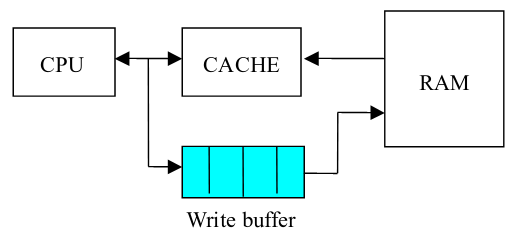
\includegraphics[width=.6\textwidth]{images/write_buffer.png}

\paragraph{Write misses}
Consists of attempts to write to an address not present in cache. Possible solutions:
\begin{itemize}
    \item \textbf{Write allocate} (also fetch on write):
    the block is allocated in cache on a write miss, and then written into the lower-level memory (according to the chosen write policy)\\
    More used by write back due to locality principle.
    \item \textbf{No write allocate} (also write around):
    the block is modified directly in lower-level memory, without being transferred to cache.\\
    More used by write through because there would be no gain in passing through cache.
\end{itemize}

\section{Improving cache performance}
Aspects to consider
\begin{itemize}
    \item Miss rate (compulsory, capacity, conflict)
    \item Miss penalty
    \item Hit time
\end{itemize}

\paragraph{Increase cache size}
Decreases miss rate but may increase hit time.

\paragraph{Larger block size to reduce miss rate}
Larger block size \textbf{reduces compulsory misses} (because of spatial locality)\\
Larger block size \textbf{increases miss penalty} (larger block to read from memory)\\
Larger block size implies fewer blocks for a fixed cache size, which \textbf{may increase conflict misses and capacity misses} (if cache is small)

\section{Split cache}
In a split cache we have two first level cache, one for the instructions and one for the data.
Statistics prove that instruction caches have lower miss rate than data caches.\\
Instruction cache: “read-mostly” – very good spatial locality\\
Data cache: locality strongly application-dependent.

\textbf{Average Memory Access Time} for split caches:
\[ AMAT = \%Instr\_references (hit\_time + miss\_rate\_I * miss\_penalty) + \
\
\%Data\_references (hit\_time + miss\_rate\_D * miss\_penalty) \]

miss\_rate\_I = miss rate for instruction cache\\
miss\_rate\_D = miss rate for data cache

\%Instr\_references = fraction of total memory references for instructions\\
\%Data\_references = fraction of total memory references for data

\paragraph{Cache locking}
some sections of cache can be locked by the programmer to be used as fast local memories.
The locked portion of cache is visible to the programmer.
The caching hardware of the locked section (e.g. tags, replacement logic)  is turned off (i.e. cache becomes a normal RAM). This is possible only with associative or set-associative caches.

\section{Multi-level cache}
The total AMAT is given by:
\[
T_A = Hit\_time_{L1} + Miss\_rate_{L1} * Miss\_penalty_{L1} \
\
= Hit\_time_{L1} + Miss\_rate_{L1} * \
\
(Hit\_time_{L2} + Miss\_rate_{L2} * Miss\_penalty_{L2}) \
\]

\subsection{Type of miss rates}
\begin{itemize}
    \item \textbf{Local miss rate}:\\
    number of misses in a cache divided by the total number of accesses to that cache
    ($Miss\_rate_{L1}$ for L1 and $Miss\_rate_{L2}$ for L2)
    \item \textbf{Global miss rate}:\\
    number of misses in a cache divided by total number of memory accesses generated by CPU
    (either $Miss\_rate_{L1}$ for L1 and $Miss\_rate_{L1} * Miss\_rate_{L2}$ for L2)
\end{itemize}

L1 and L2 caches should be different to improve overall performance.

\subsection{Inclusion vs exclusion policies}
\begin{itemize}
    \item \textbf{Multilevel inclusion}:\\
    L1 data always present in L2 (it ensures consistency between I/O and caches). \textit{Problem}: performance analysis suggests that L1 blocks may be smaller than L2 ones so that substitution might become difficult.
    \item \textbf{Multilevel exclusion}:\\
    L1 data are never found in L2. Reasonable if L1 and L2 have similar size
\end{itemize}

\subsection{Split vs unified}
Performance analysis showed that the best approach is to use
\begin{itemize}
    \item L1 cache: Split\\
    High bandwidth for simultaneous data and instruction access.
    Separate optimization
    \item L2 cache: Unified\\
    Reduced area size. Better flexibility on memory usage
\end{itemize}

\subsection{Write policy}
\begin{itemize}
    \item L1 cache: Write through + no-write-allocate\\
    Avoids problems with coherence in L1. Simpler implementation for on-chip solution
    \item L2 cache: Write back + write-allocate\\
    Reduces overall bus traffic. Captures temporal and spatial locality
\end{itemize}

\subsection{Block size}
A larger block size assures a better use of spatial locality.
Compulsory misses decrease. Conflict and capacity misses may increase, since larger blocks means fewer blocks in cache. However, miss penalty increases so there would be a higher access time.

\subsection{Degree of associativity}
\begin{itemize}
    \item L1 cache: No clear winner\\
    DM: faster cycle time, lower hit rate\\
    Set associative: longer hit-time vs. better hit rate
    \item L2 cache: No clear winner\\
    Set-associative less advantageous for really large caches\\
    Set-associative L2 gives flexibility
\end{itemize}

\paragraph{Critical Word First}
request missed word from memory, send it to CPU as soon as it arrives; CPU runs while the rest of the cache block is filled (also called wrapped  fetch, request word first).

\paragraph{Early restart}
words are fetched in normal order, as soon as the requested one arrives it is sent to the CPU.

\paragraph{Victim cache}
A small, fully associative cache (victim cache) can be inserted between cache and its refill path; Victim cache contains only blocks discarded from cache on a miss (victims) that are checked on a miss before going to lower-level memory.\\
If requested data are in victim cache, victim block and cache block are swapped.

\section{Virtual Memory}
Computers run multiple processes, each with its own address space.
Can’t give each process a full address space worth of memory.

The solution is to divide physical memory into blocks and allocate them to different processes.
Need a protection scheme so that processes can access only their blocks.

Virtual memory also useful to offload to secondary storage (disks) parts of (block) programs and data that can’t fit in main memory. The swapping between main memory and secondary storage is automatically managed by the operating system.

Process sees a virtual address space. 
Blocks in virtual space are allocated anywhere in physical memory or in secondary storage.

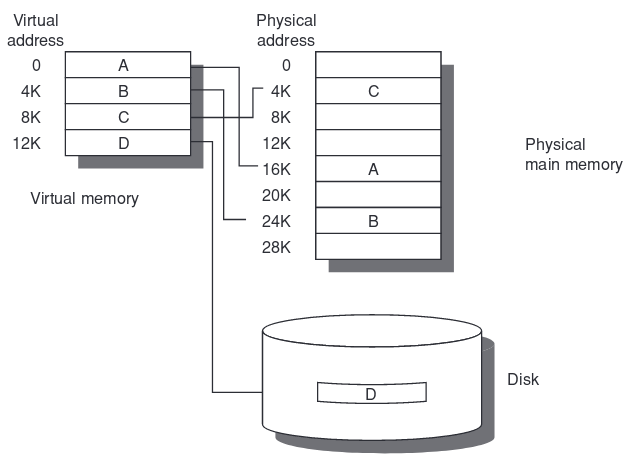
\includegraphics[width=\textwidth]{images/virtual_memory_scheme.png}

Similar to caches: 
blocks usually called pages or segments
and misses are called page faults.

The virtual address generated by the process must be translated into the physical address. It's called memory mapping or address translation.

\subsection{Differences with caches}
\paragraph{Replacement}
\begin{itemize}
    \item Caches: controlled by the hardware
    \item Virtual memory: controlled by the operating system. The high miss penalty means it is more important to make a good replacement!
\end{itemize}

\paragraph{Size}
\begin{itemize}
    \item Processor address bus size determines size of virtual memory
    \item Cache size independent of processor address bus size
\end{itemize}

\paragraph{Secondary storage}
Also used for file system

Blocks can be placed anywhere in main memory, it's like a \textbf{fully associative} cache.

On a page fault for replacing a block most operating systems use \textbf{LRU}.

For writing a page all virtual memory systems use \textbf{write-back}.

To search a block in main memory it is used a table to record correspondence between virtual page number and physical address.
Sometimes a hash table is used, the size of the actual number of pages in physical memory in use.

\paragraph{Fast address translation}
Page tables are usually large so are stored in main memory and paged.
2 memory accesses are needed: one for translation, one for data.

Address translation uses a special fully associative cache: \textit{Translation lookaside buffer (TLB)}

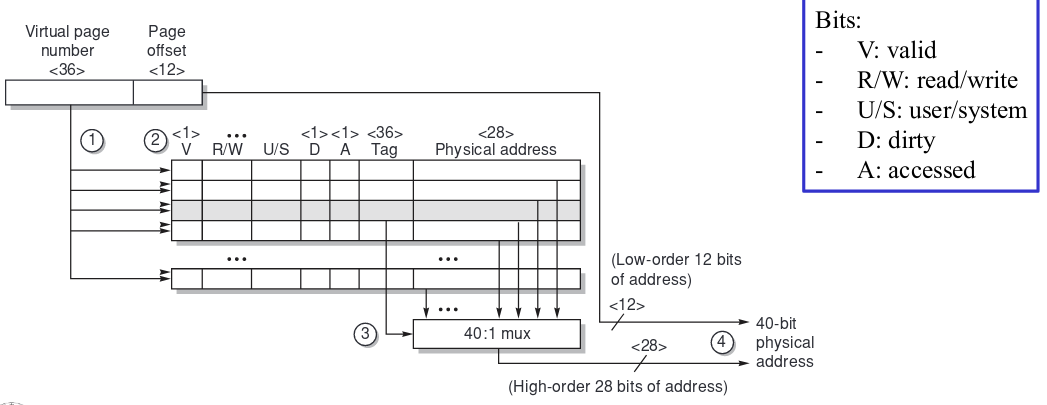
\includegraphics[width=\textwidth]{images/TLB_scheme.png}

\section{A Dynamic RAM (DRAM) cell}
In most dynamic memories 1 cell consists of just 1-transistor as a storage capacitor $C_i$.
Charge sharing with bit line capacitance ($C_i << C_{BL}$).
Due to leakage currents, memory cell content must be refreshed periodically.

Reading much slower than writing because it implies 3 operations:
\begin{itemize}
    \item Precharge
    \item Reading
    \item Write back
\end{itemize}
DRAM much slower than SRAM and it is also more power hungry.

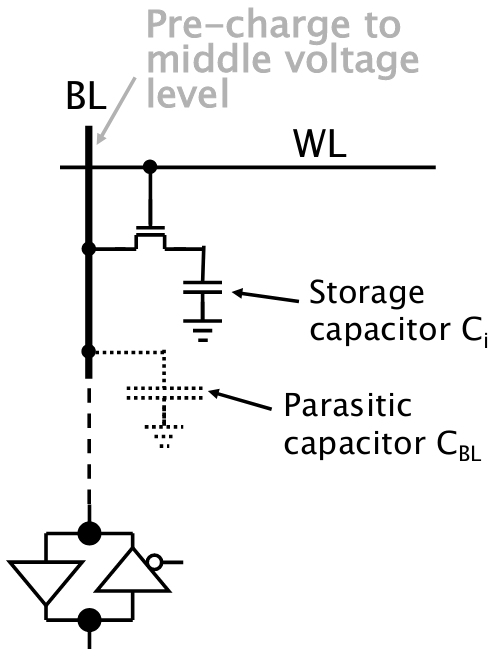
\includegraphics[width=.4\textwidth]{images/DRAM_scheme.png}

\section{"Typical" memory structure}
The SRAM memory has usually a cell array layout.

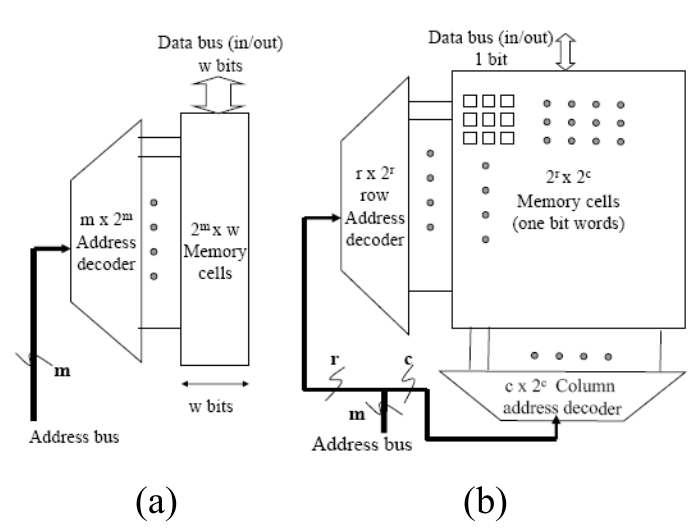
\includegraphics[width=\textwidth]{images/SRAM_scheme.png}

Ideally it should be linear (a), but this approach is not suitable:
\begin{itemize}
    \item Long data bus so large capacity
    \item Address decoder will have a lot of logic levels
    \item Memory layout too long and thin
\end{itemize}

It is better to split the m-bit address into an r-bit row address and a c-bit column address (b). 
We reach smaller decoders, almost square memory layout, faster architecture (lower WL and BL delays)

\section{DDR commands}
\begin{itemize}
    \item \textbf{PRECHARGE}\\
    Close current row, get ready for an activate
    \item \textbf{ACTIVATE (RAS)}\\
    Open a row and store row result in a register.
    Row is open until next precharge command.
    \item \textbf{READ (CAS)}\\
    Read values from open row
    \item \textbf{WRITE (CAS)}\\
    Write values to open row
    \item \textbf{REFRESH}\\
    Restore values in rows (essentially a periodic ACTIVATE)
\end{itemize}

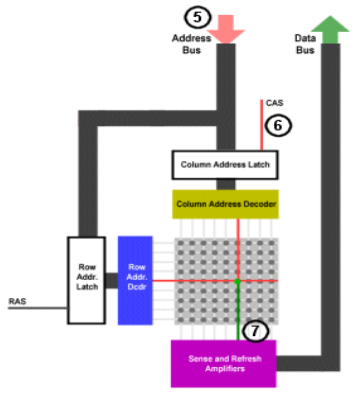
\includegraphics[width=.6\textwidth]{images/DRAM_memory_structure.png}
\begin{enumerate}
    \item The row address is placed on the address pins via the address bus
    \item The Row Access Strobe (RAS) is activated, which places the row address onto the Row Address Latch
    \item The Row Address Decoder selects the proper row to be sent to the sense amps
    \item The column address is placed on the address pins via the address bus
    \item The Column Address Strobe (CAS) is activated, which places the column address on the Column Address Latch
    \item The CAS pin also serves as the Output Enable, so the sense amps place the data from the selected row and column on the Data Out pin
\end{enumerate}

\section{Synchronous DRAM (SDRAMs)}
\begin{itemize}
    \item A specific CLK signal is transmitted over a dedicated control line
    \item Communication times are based on a multiple of the clock period
    \item Commands are sent and managed like in a pipeline
    \item Burst transfer(i.e. transfer of chunks of data after a single addressing phase) are possible
    \item In double data rate (DDR) SDRAM memories, both clock edges are used to transfer data
\end{itemize}

\section{Magnetic Disks}
\begin{itemize}
    \item \textit{Cylinder}: all the tracks under the arms at a given point on all surfaces.
    \item \textit{Seek time (Ts)}:time to move the arm to the desired track (5-12 ms on average)
    \item \textit{Rotation latency(or delay) (Tr)}: time for the requested sector to rotate under the head. The average latency to the desired information is obviously halfway around the disk (3-5 ms)
    \item \textit{Transfer time (Tt)}: time to transfer a block of bits, typically a sector, under the read-write head. This time is a function of the block size, disk size, rotation speed, recording density of the track, and speed of the electronics. A disk buffer (4-16 MB) can improve Tt by exploiting spatial locality
    \item \textit{Controller time (TC)}: overhead the disk controller imposes in performing an I/O access 
\end{itemize}

$Access\_time = T_s + T_r + T_t + T_c$

